\documentclass[journal]{IEEEtran}
\usepackage{epsf,cite,amsmath,amscd,graphics,graphicx,latexsym,multicol,setspace}
\usepackage{amsfonts,amsmath,amssymb,amsthm}
\usepackage{scalefnt}
\usepackage{cuted}
\usepackage{flushend}
\usepackage[justification=centering]{caption}
\usepackage{subcaption}
\newcounter{MYtempeqncnt}
\begin{document}
\title{Low-Dose CT Image denoising and Restoration using General Adversarial Networks}

\author{Kevin Freire $|$ kfreirea@ryerson.ca\\
Walter Freire $|$ andrei.freire@ryerson.ca \\
Department of Electrical and Computer Engineering\\
Ryerson University, Toronto, Canada.}
\maketitle

% ABSTRACT
\begin{abstract}
Medical Imaging has been a growing topic in computer vision for its life saving applications.  Medical professionals rely on good quality images of their medical scans in order to correctly identify tumours or other anomalies.  Recent studies have shown that Computerize Tomography CT scans have great results using high radiations for their X-Rays.  Studies have shown that these (CT) Scans have produced more than half the radiation from medical use which results in problems for long term use of these expensive machines.  Some solutions have involved reducing the X-Ray magnitude in order to reduce exposure to X-Ray but this results in lower quality images with a lot of noise.  We implemented a denoising neural network trained on medical images to reduce the noise from low dose CT Scans.  This model is capable of producing high dose quality imaging using low dose CT Scans at a reasonable rate.  We have implemented our approach and version of our code can be obtained from https://github.com/kevinfreire/ldct-denoising.
\end{abstract}

% KEYWORDS
\begin{IEEEkeywords}
Image restoration, Image Denoising, General Adversarial Networks, GANs, Low-Dose CT, Medical Imagery, Deep Neural Networks.
\end{IEEEkeywords}

% INTRODUCTION
\section{Introduction}
\label{Introduction}
Computerize Tomography (CT) has enabled direct imaging on the 3-dimensional structure of different organs and tissues inside the human body in a non-invasive manner. CT scans are constructed by combining the X-ray scans taken on several angles and orientations.  It has several utilities but very useful in detecting lesions, tensions, tumours, and metastasis.  It can reveal their presence and the spatial location, size and extent of the tumour.  CT imaging has become a frequent tool for cancer diagnosis, angiography, and detecting internal injuries.  However, despite the evidence of its utility for diagnosis and patient management, the potential risk of radiation-induced malignancy exists \cite{brenner2007computed}.  Studies found that CT alone contributes to almost half of the total radiation exposure from medical use alone.  Recent studies reveal that as much as 1.2 - 2\% of cancers may eventually be caused by the radiation dose conceived by the patient while undergoing CT scans \cite{schauer2009national}.  To reduce the risk, the principles of ALARA (As Low As Reasonably Achievable) is now a profound practice predicted in CT imaging \cite{protection2007icrp}.  In regards to this practice, Low Dose CT (LDCT) is a promising solution in reducing radiation exposure \cite{trattner2014standardization}.  In low dose CT, radiation exposure is decreased by lowering the tube current, or voltage.  However, by reducing the tube voltage or current it introduces several artifacts and lowers the diagnostic quality of the LDCT image \cite{boas2012ct}.  In order to boost the quality of an LDCT image, the reconstruction of LDCT has become a primary research.  There are various methods that can be classified under three categories: (a) iterative reconstruction, (b) sinogram filtration based techniques, and (c) image post-processing based technique.  In recent times, researchers were trying to develop new iterative algorithms (IR) for LDCT image reconstruction.  Iterative reconstruction algorithms considerably suppresses the image noise, but still lose some details and suffer from remaining artifacts.  Other disadvantages with IR techniques is the high computational cost, which is a bottle neck in practical utilization.  Sinogram filtration on the other hand, directly works on the projection data before reconstructing the image and is more computationally economical than the IR technique.  However, the data of commercial scanners are not readily available to users, and this method suffers from edge blurring and the resolution loss.  Many efforts were made in the image domain to reduce LDCT noise and suppress artifacts.\\
With the explosive evolution of deep neural networks, the LDCT denoising task is now dominated by deep neural networks.  However, the research on deep learning-based LDCT denoising is confined to designing a network architecture based on the vanilla convolution operation.  There has been a surge in interest in designing General Adversarial Networks (GAN), mainly for image generation and becoming popular in denoising medical images as shown in \cite{8340157}, \cite{9474492}, \cite{yin2021unpaired}.  In this paper we explore the possibility of applying GAN to the task of LDCT denoising.\\
	In many image-related reconstruction tasks, it is known that minimizing the per-pixel loss between the output image and the ground truth alone generate either blurring or makes the result visually unappealing \cite{huang2017beyond}.  The same effect was observed in the traditional neural network-based CT denoising works \cite{chen2017low}, \cite{chen2017low2}.  The adversarial loss introduced by GAN can be treated as a driving force to push the generated image to look as close to as the groung truth image or in this case the Normal Dose CT image (NDCT) which also reduces the blurring effect. Further more, an additional perceptual loss was also introduced to measure the feature of the denoised image, with a focus on areas that the human eye cannot see. \\
Generative Adversarial Network was first introduced in 2014 by Goodfellow \emph{et al}. \cite{goodfellow2014generative}.  It is a generative model trying to generate real world images by employing a min-max optimization framework where two networks (Generator G and Discriminator D) are trained against each other.  G tries to synthesize real appearing images from random noise wheras D is trying to distiguish between the generated and real images.  If the Generator G get sufficiently well trained, the Discriminator D will eventually be unable to tell if the generated image is fake or not.\\
	The original setup of GAN does not contain any constraints to control what modes of data it can generate.  However, the auxiliary information were provided during the generation, GAN can be driven to output images with specific modes.  In this scenario, GAN is usually referred to as conditional GAN (cGAN) since the output is conditioned on additional information.  Bera \emph{et al}. \cite{9474492} proposed a discriminator function for CT denoising task, which leverages self-attention and pixel-wise GANs for restoring the diagnostic quality of LDCT images.  Yi \emph{et al}. \cite{yi2018sharpness}. proposed an adversarial trained network and a sharpness detection network to denoise LDCT images. Both \cite{8340157} and \cite{yin2021unpaired} used Wasserstein GAN with Perceptual Loss and Wasserstein Distance to generate a denoised image of an LDCT image. \\
	In this paper, we make the following contributions:
	
	\begin{enumerate}
		\item We built a GAN architecture similar to Alsaiari \emph{et al}. \cite{alsaiari2019image}. with the exception of training it specifically on LDCT images.
		\item Computed similar loss functions as \cite{alsaiari2019image}, with the exception of using the Mean Squared Error Loss function instead of computing L2-norm.
		\item Present the output results of the network after training.
	\end{enumerate}
	
 The remainder of this paper is organized as followed.  The proposed method based on \cite{alsaiari2019image}, with perceptual loss, pixel-pixel loss, smooth loss and adversarial loss are presented in \ref{method}.  Then, experiments and analysis of the results are presented in section \ref{experiment settings} and \ref{results and discussion}.  Lastly, Section \ref{conclusion} gives a summary of this paper and looks forward to some possible future research directions.

% METHOD
\section{Method}
\label{method}
	We built a GAN network structure for image denoising, which like, \cite{alsaiari2019image}, is based on ResNet \cite{he2016deep}.  A generator network is trained to generate noise free images through competition with the discriminator network, using ground truth NDCT images to improve the quality of the generated images.  Our network makes use of residual blocks, skip connections, and batch normalization.  Due to training limitations, we used three residual blocks.  However, having a larger number of residual blocks would increase the training accuracy significantly, but with a higher computational complexity and longer training times.\\
	Suppose that $z \in \{z_k\}_1^N$ denotes the LDCT image, $x \in \{x_k\}_1^N$ denotes the NDCT image, and $p_l$ and $p_r$ represent the distribution of LDCT and NDCT images, respectively.  The generator G learns a mapping $G: z \rightarrow \hat{x}$, where \emph{z} is the LDCT the generator is conditioned upon.  $\hat{x}$ is the denoised CT that is expected to be as close to as the NDCT image \emph{x}.  The discriminator D, is to differentiate the generated image \emph{z} from the real \emph{x}.  
	
\begin{figure*}[t!]
    \centering
    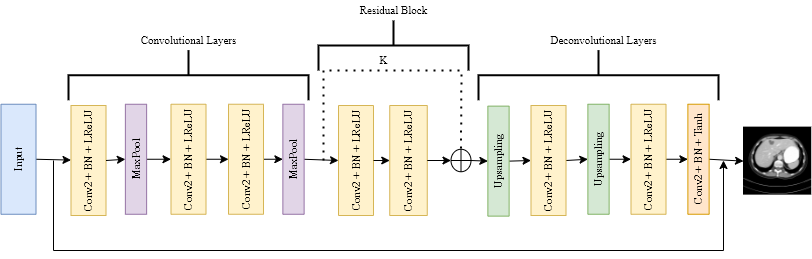
\includegraphics[width=15cm]{generator}
    \caption{Generator Network Architecture with $K=3$}
    \label{generator}
\end{figure*}	
	
% LOSS FUNCTION
\subsection{Loss Function}
\label{loss function}
In the original GAN \cite{goodfellow2014generative}, D and G are trained by solving the following minmax problem

\begin{equation}
	\mathop{min}_{G}\mathop{max}_{D} L_{GAN}(D,G) = -E_{x \tilde p_r}[D(x)] + E_{z \sim p_l}[1-D(G(z))]
\end{equation}

where $E(\cdot)$ denotes the expectation operator, $G(\cdot)$ and $D(\cdot)$ represents the outputs of G and D.  The generator G transforms a noisy sample to mimic a real sample, which defines a data distribution, denoted by $p_g$.  Then D is trained to become an optimal discriminator for a fixed G, the minimization search for G is equivalent to minimizing the Jensen-Shannon (JS) divergence of $p_r$ and $p_g$, which will lead to a vanished gradient on the Generator G  \cite{8340157} and G will stop updating as the training continues.  \\
	In the process of using CT image training, the feature difference between the LDCT and NDCT image will have a certain probability of structural loss in denoising results.  In order to obtain a good quality image, we include the Minimum Square Error Loss (MSE) between the Generated image $\hat{x}$ and the ground truth $x$.  The function is expressed as follows:
	
\begin{equation}
	L_{MSE} = E_{z\sim p_l}\left[ \frac{1}{N}\|x - G(z)\|^2 \right],
\end{equation}
	
Where $\|\cdot\|^2$ is the square L2-norm (MSE Loss).  A lower difference denotes a higher quality of the generated image.  However, the MSE loss can potentially generate blurry images and cause the distortion or loss of details.  Thus, we also applied the perceptual loss.\\
	With perceptual loss, the rational behind it is two-fold.  First, when a person compares two images, the perception is not performed pixel-by-pixel.  The human vision extracts and compares features from images \cite{nixon2019feature}.  With perceptual loss, it guides the model towards image style conversion \cite{johnson2016perceptual}, image denoising \cite{8340157}, and other tasks.  The perceptual loss function is introduced to learn feature distribution of NDCT images from the feature space to guide the denoising task of LDCT images.  Therefore, we included a pre-trained deep CNN (VGG16) for feature extraction and compared the denoised output against the ground truth in terms of the extracted features.  The perceptual loss function is defined in a feature space:
	
\begin{equation}
	L_{Perceptual}(G) = E_{(x,z)}\left[ \frac{1}{whd}\|\Phi(G(z))-\Phi(x)\|^2 \right],
\end{equation}

	where $\Phi$ is the feature map obtained from the output of the second convolutional layer of the VGG-16 pretrained network, $G(z)$ is the denoising result of the LDCT image, \emph{w}, \emph{h}, \emph{d} represents width, height and depth of the feature map, respectively.  It should be noted that we used the VGG-16 network as the feature extractor.  The input of the network is a colour image, including three channels, while the CT images is greyscale image.  Thus, before using the network for feature extraction, we duplicated the CT image to make RGB channels.\\
	We also added a smooth loss function to the existing loss functions and the intuition behind this is to prevent the ``check-board'' artifacts across neighbouring pixels in the image.  The smooth loss function is defined as followed:

\begin{equation}
	L_{Smooth} = \left[ \frac{1}{N_x}\|\hat{x}_x - \hat{x}_{x+1}\|^2 \right]+ \left[ \frac{1}{N_y}\|\hat{x}_y - \hat{x}_{y+1}\|^2 \right]
\end{equation}

	where $\hat{x}_x$, $\hat{x}_y$ is the generated image in the x-direction and y-direction and $\hat{x}_{x+1}x$, $\hat{x}_{y+1}$ are the generated image shifted to the right and downward respectively.
	Combining all the loss functions we then defined the new loss function as follows:
	
\begin{equation}
	L_{Net} = \lambda_a L_{GAN} + \lambda_m L_{MSE} + \lambda_p L_{Perceptual} + \lambda_s L_{Smooth},
\end{equation}

where $\lambda_a, \lambda_m, \lambda_p$ and $\lambda_s$ are pre-defined weights for adversarial loss, MSE loss, Perceptual loss and smooth loss, respectively.

% GENERATOR NETWORK
\subsection{Generator Network}
\label{generator}
The goal of a single image denoising is to generate a realistic image with high quality.  The generator fills in the noises or reduces noise with neighbouring pixels without loosing information present in the original image.  We adopted a structure similar to \cite{alsaiari2019image}, however we added \emph{max pooling layers} and \emph{upsampling layers}.  This is similar to a traditional CNN framework, that directly learns an end-to-end mapping from input noisy image to their corresponding ground truth.  A set of three convolutional layers, using batch normalization, and \emph{LeakyReLU} activation, are stacked in the front of the network with two \emph{maxPooling} layers, one after the first convolution layer and after the third convolution layer, this extracts semantic attributes from the input image.\\
	Three residual blocks are stacked after the convolutional layers.  Each residual block contain two convolutional layers which increases the depth of the network.  A symmetric skip connection is involved to improve efficiency in training and to promote faster convergence.  The skip connections feed the input to the deep layers so each residual layer tune the output with reference to the input and retains spatial information.  These are followed by three ''deconvolution'' layers, each corresponding to \emph{upsampling} layers and convolutional layers in the front of the network.   The images are resize from $30 \times 30$ to $60 \times 60$, and the final image output is a size of $120 \times 120$.  Note that we stated the last three layers as \emph{deconvolutional} for simplicity, however in fact a deconvolutional layer does not actually use upsampling operation.  The first two deconvolution layers have \emph{LeakyReLU} activations and the final layer providing the denoised output has a \emph{Tanh} activation.  For all layers we use a stride of 1.  The generator network is shown on Figure \ref{generator} where \textbf{k} stands for the kernel size, \textbf{n} is the number of output channels and \textbf{s} is the stride. 

\begin{figure*}[th!]
    \centering
    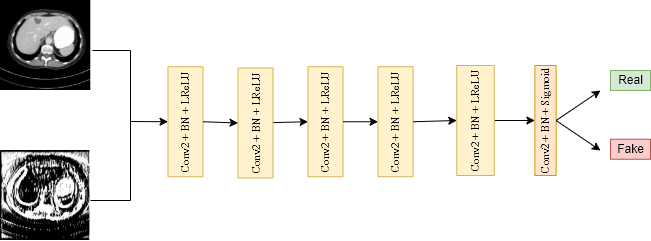
\includegraphics[width=10cm]{discriminator}
    \caption{Discriminator Network Architecture}
    \label{discriminator}
\end{figure*}

% DISCRIMINATOR NETWORK
\subsection{Discriminator Network}
\label{discriminator}
	What makes a GAN network very unique is the critic network or Discriminator network.  The only purpose for the discriminator is to classify each input image as real or fake.  Similar to \cite{alsaiari2019image}, we use five convolutional networks with Batch normalization and \emph{LeakyReLU} activation throughout the network.  Once the network learns from a set of these conv-BN-LReLU, a sigmoid function is stacked at the end to map the output to a probability score normalized to $[0,1]$.  The structure of the Discriminator is shown in Figure \ref{discriminator} where \textbf{k} stands for the kernel size, \textbf{n} is the number of output channels and \textbf{s} is the stride.

% EXPERIMENT SETTINGS
% this section includes dataset and training details
\section{Experiment Settings}
\label{experiment settings}
	The network was trained using Google Colab Pro which use a K80 GPU and 24 GB of RAM using the Pytorch framework. We used a batch size of 16,  and ran over 15000 iterations for training which was around 500 epochs.  For validation of our experiment algorithm, we used the publicly available dataset from the Cancer Imaging Archive of 10 patients taken in 2018\footnote{https://www.cancerimagingarchive.net/}.  For each patient there was an average of 173 slices pre patient.  We used images from 9 patients as the training set and images from 1 patient as the test set.  Our test set had more than 400 image pairs.  For training, we have taken 10 randomly cropped patches from each slice, each patch size $120 \times 120$.  For training our network, we used a similar approach as \cite{9474492} setting the Adam optimizer with batch size of 16.  The learning rate was initially set to $1e^{-4}$ for generator network and $4e^{-4}$ for the discriminator network, and was set to decrease by a factor of 2 after every 6000 iterations.  During training we set different hyper parameters which include $\lambda_a=0.5$, $\lambda_m=1.0$, $\lambda_p=1.0$ and $\lambda_s=0.0001$. We set $K=32$ and $k_2=48$ for the generator and discriminator channel filters.  For the convolutional and deconvolution layers of the generator we used a kernel size of 9 and stride 1.  All the other convolutional layers in the generator had a kernel size of $3 \times 3$ and stride 1.   The discriminator first 3 layers, all of its convolutional networks had a $4 \times 4$ kernel size with stride 2 and zero padding by 1.  the last two layers in D are composed of kernels of size $4\times 4$ with stride 1 and zero-padding of 1. To train the discriminator and generator we took the approach of training one at a time.  We did this by training the discriminator first for 2 epochs and then training the generator for 10 epoch, then the cycle repeats.  We trained the network until there was no further improvement in reconstruction loss.  We have implemented our approach and version of our code can be obtained from https://github.com/kevinfreire/ldct-denoising.
	
\begin{figure*}
     \centering
     \begin{subfigure}[t]{0.22\textwidth}
         \centering
         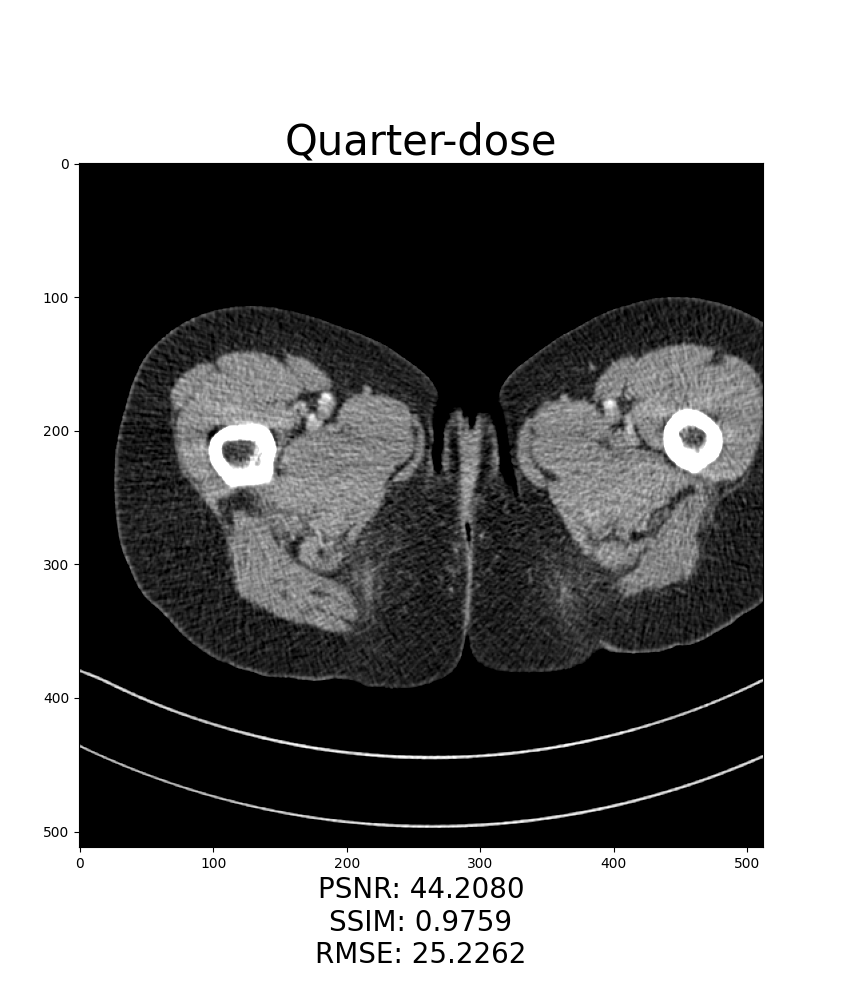
\includegraphics[width=\textwidth]{ldct}
         \caption{low-dose image}
         \label{ldct}
     \end{subfigure}
     \begin{subfigure}[t]{0.22\textwidth}
         \centering
         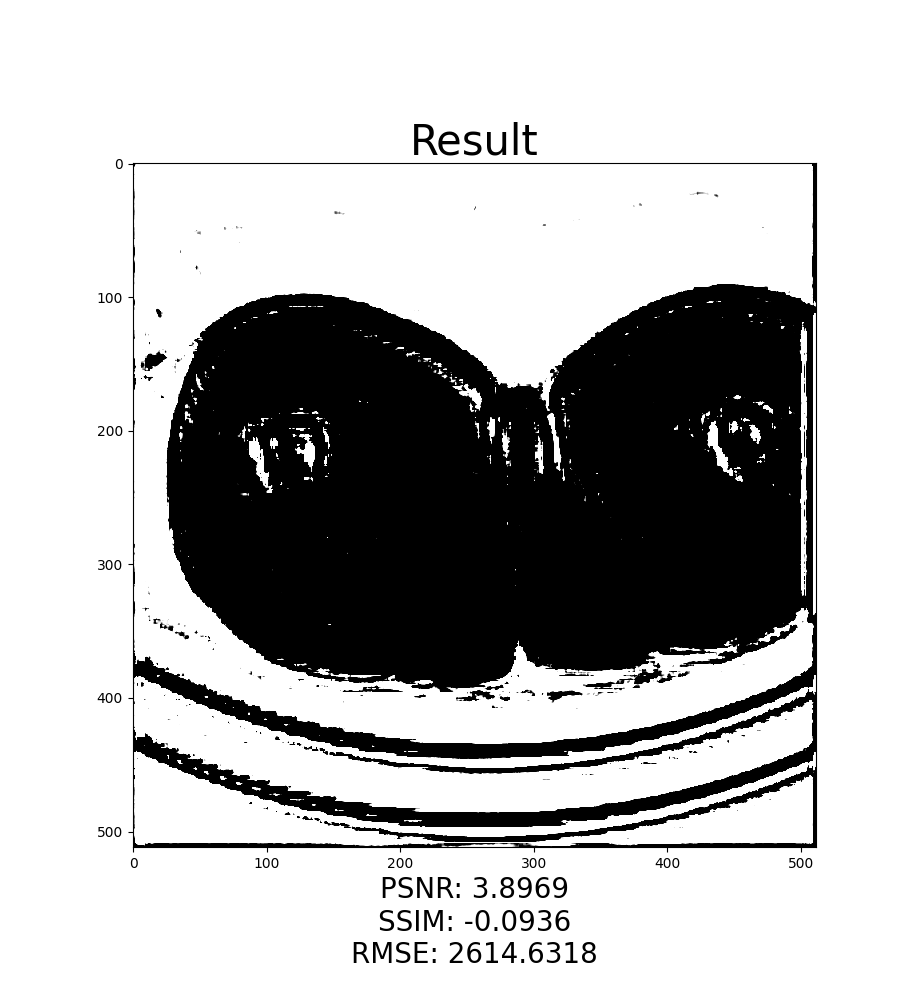
\includegraphics[width=\textwidth]{epoch0}
         \caption{Generated image at epoch 0}
         \label{epoch0}
     \end{subfigure}
     \begin{subfigure}[t]{0.22\textwidth}
         \centering
         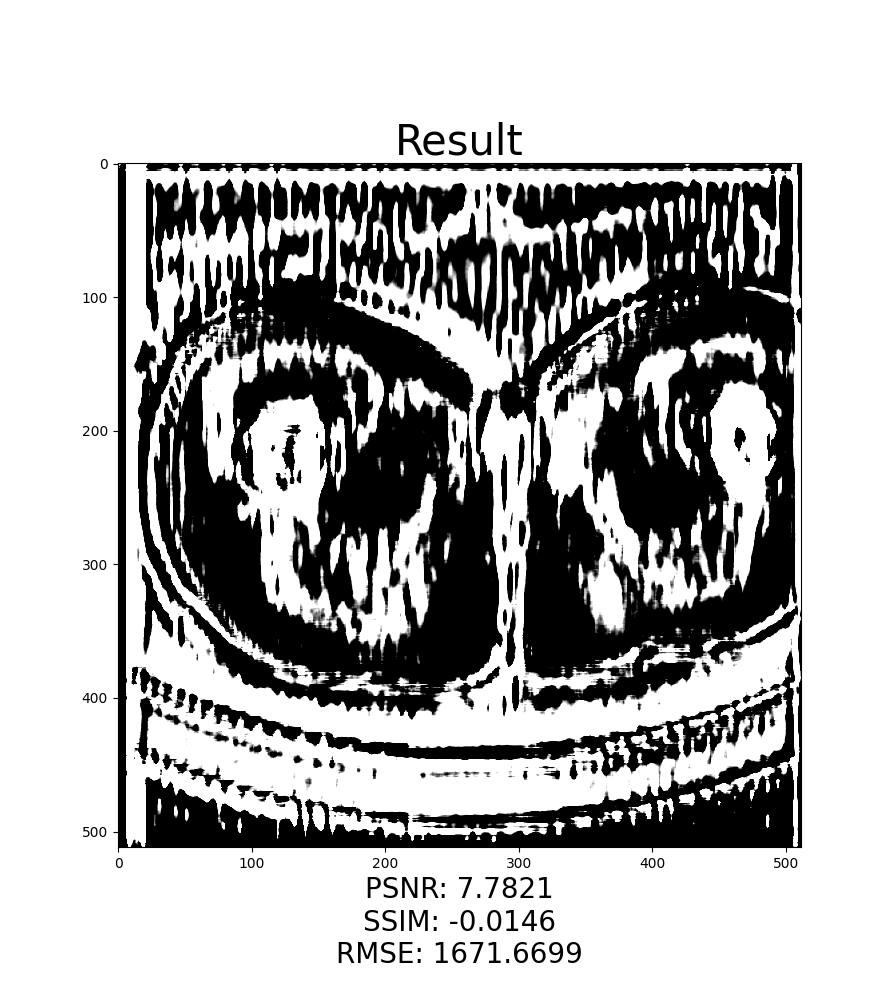
\includegraphics[width=\textwidth]{epoch10}
         \caption{Generated image at epoch 10}
         \label{epoch10}
     \end{subfigure}
     \begin{subfigure}[t]{0.22\textwidth}
         \centering
         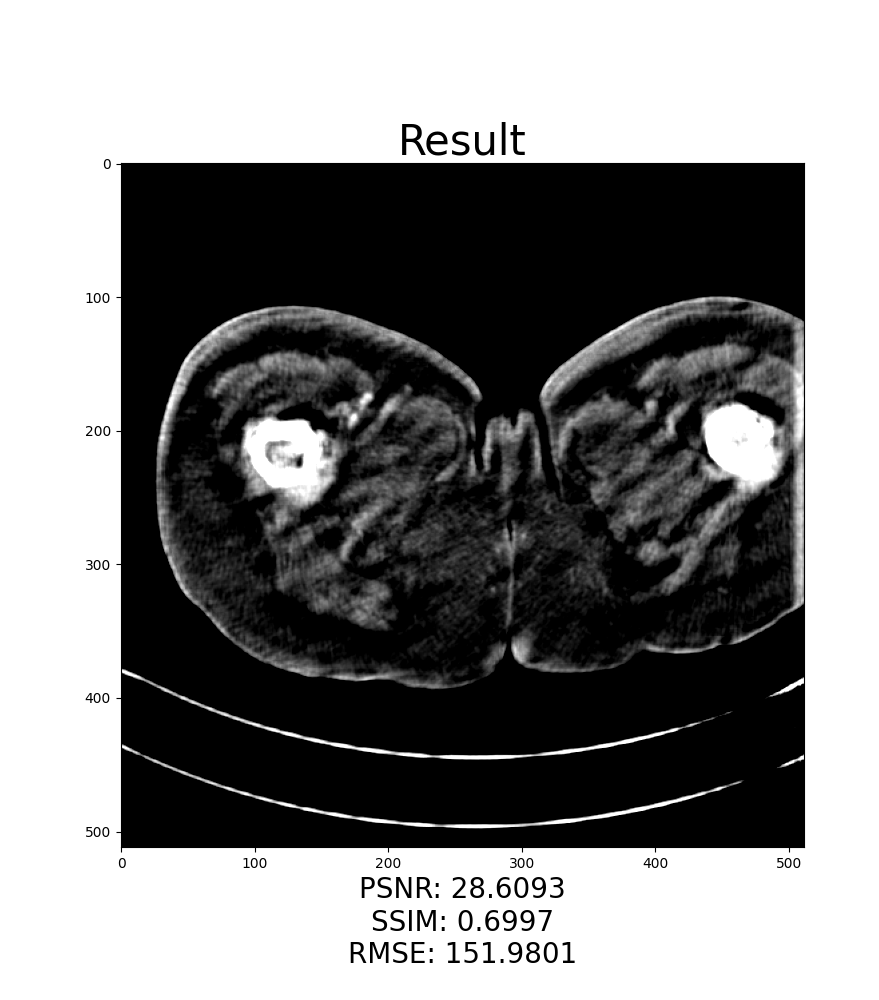
\includegraphics[width=\textwidth]{epoch100}
         \caption{Generated image at epoch 100}
         \label{epoch100}
     \end{subfigure}
     \begin{subfigure}[t]{0.22\textwidth}
         \centering
         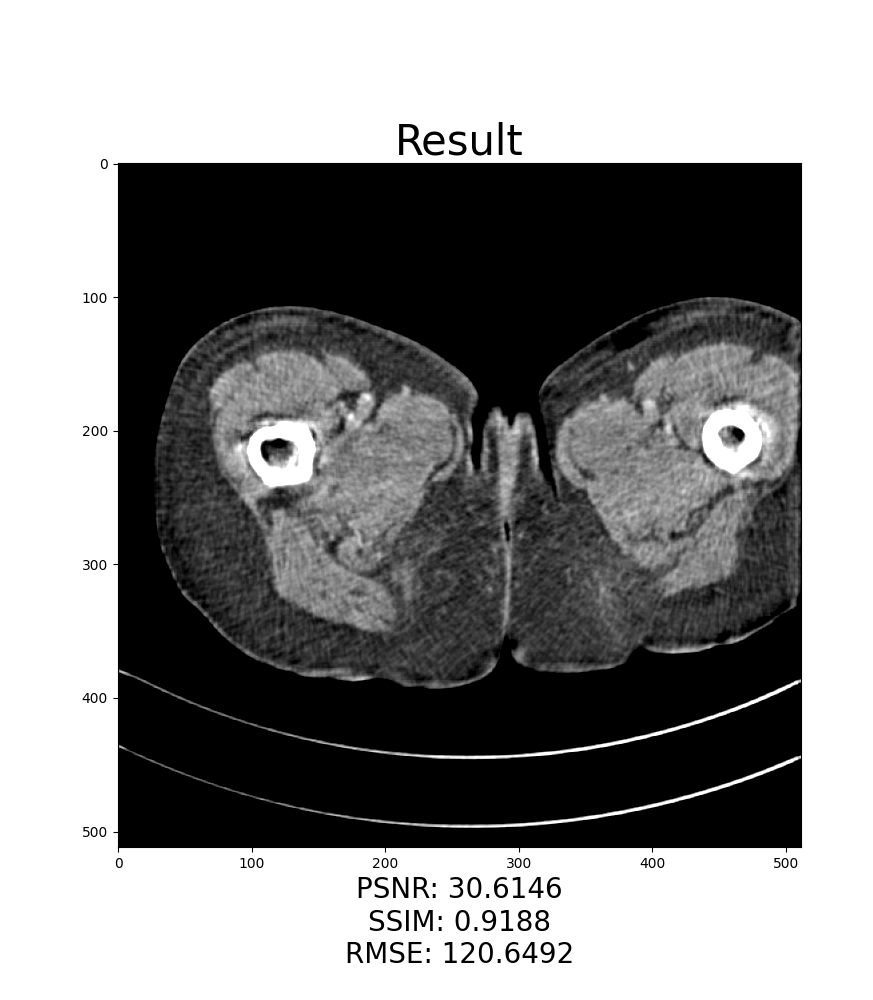
\includegraphics[width=\textwidth]{epoch160}
         \caption{Generated image at epoch 160}
         \label{epoch160}
     \end{subfigure}
     \begin{subfigure}[t]{0.22\textwidth}
         \centering
         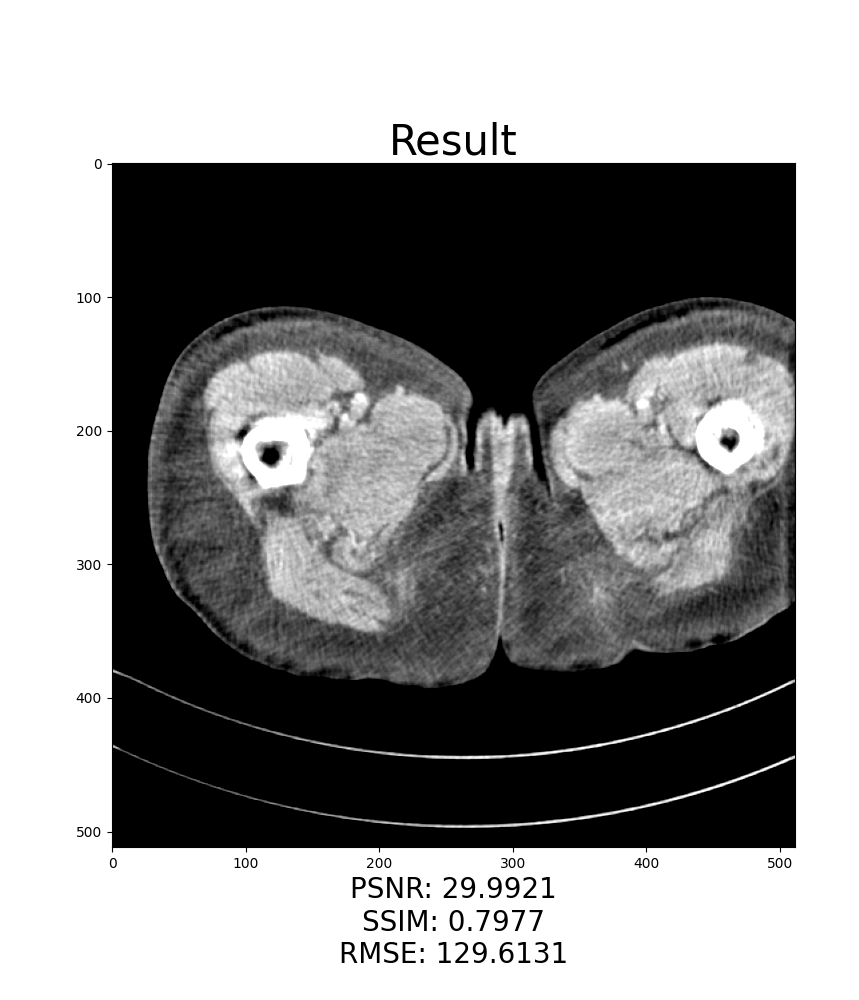
\includegraphics[width=\textwidth]{epoch180}
         \caption{Generated image at epoch 180}
         \label{epoch180}
     \end{subfigure}
     \begin{subfigure}[t]{0.22\textwidth}
         \centering
         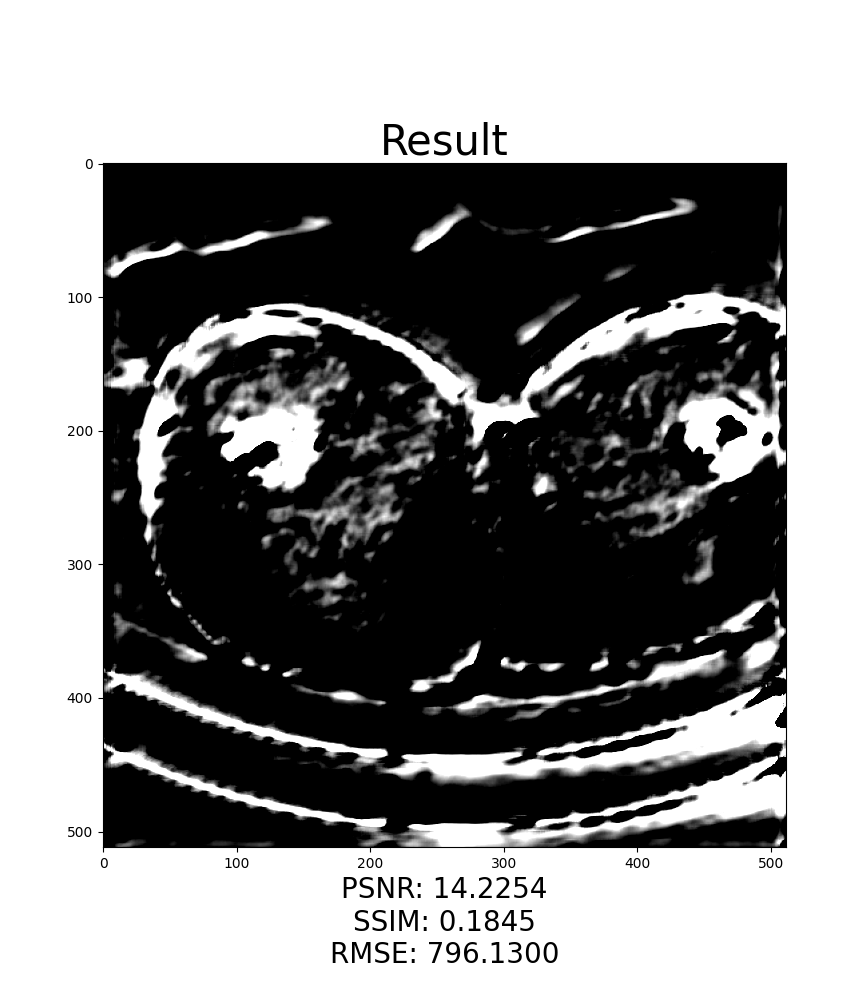
\includegraphics[width=\textwidth]{epoch200}
         \caption{Generated image at epoch 200}
         \label{epoch200}
     \end{subfigure}
     \begin{subfigure}[t]{0.22\textwidth}
         \centering
         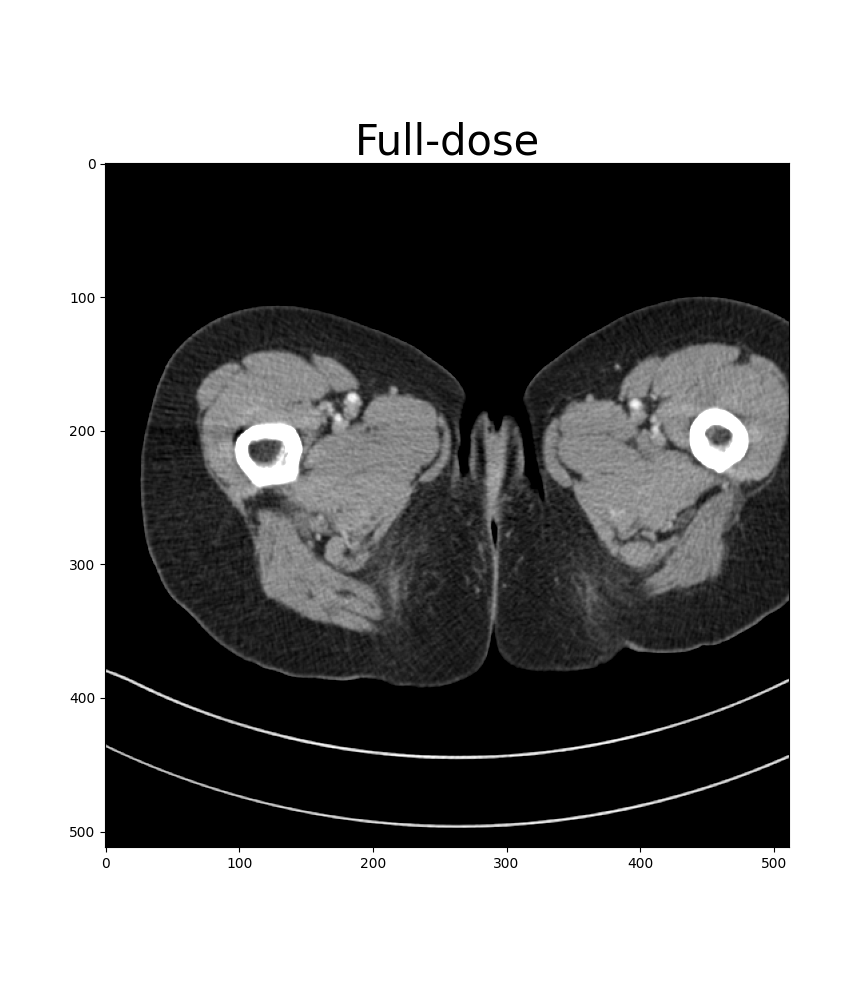
\includegraphics[width=\textwidth]{fulldose}
         \caption{full-dose image}
         \label{fulldose}
     \end{subfigure}
        \caption{GAN training process through different epochs}
        \label{GANtraining}
\end{figure*}

% RESULTS AND DISCUSSIONS
\section{Results and Discussion}
\label{results and discussion}
Due to computational limits, we were unable to compare other state-of-the-art models with ours.  What we did during training is we saved the model every 10 epochs, which was not the best thing to do and it will be discussed soon.  Since we do not have model comparisons, the results will be compared in terms of epochs.  As stated before, the Generator only generates images and attempts to generate images to fool the discriminator.  Building a GAN model is tricky and if not designed correctly, it can be unstable.  In our case our GAN model was not successful in denoising the image, however it was improving and once it passed 160 epochs the Generator started to generate poor quality images.  By observing Figure \ref{GANtraining} it is evident that the network is slowly learning as shown in Figures \ref{epoch0} - \ref{epoch160} and once it passes epoch 160 it stops learning and starts to forget how to generate denoised images as shown in Figures \ref{epoch180} - \ref{epoch200}.  In order to demonstrate the denoising performance of the model based on the training data, we compared results of other epoch training  results in Table \ref{comparison}.  

\begin{table}[h!]
\centering
\caption{Comparison of Measurements Throughout Training.}
\label{comparison}
	\begin{tabular}{ |p{1.5cm}|p{1.5cm}|p{1.5cm}|p{1.5cm}|  }
	\hline
	\multicolumn{4}{|c|}{\textbf{Measurement}} \\
	\hline
	Epoch & PSNR & RMSE & SSIM \\
	\hline
	NDCT & 44.2080 & 0.9759 & 25.2262\\
	0 & 3.8969 & -0.0936 & 2614.6318\\
	10 & 7.7821 & -0.0146 & 1671.6699\\
	100 & 28.6093 & 0.6997 & 151.9801\\
	160 & 30.6146 & 0.9188 & 120.6492 \\
	180 & 29.9921 & 0.7977 & 129.6131\\
	200 & 14.2254 & 0.1845 & 796.1300\\
	\hline
	\end{tabular}
\end{table}

Moreover, we used three different metrics to compare which include the root mean square error (RMSE), peak-signal-to-noise ratio (PSNR) and structural similarity index measure (SSIM) for our quantitative assessment of the image quality.  The goal in terms of metric is to achieve a high PSNR (preferable higher than the LDCT image), a low RMSE value (if it's zero that means it's a perfect denoised image), and an SSIM of 1.  However, it is highly likely that any state-of-the-art model can achieve a perfect denoised image.  Moreover, by observing Table \ref{comparison} it is evident that the model was in fact training and improving however, it reach a threshold and eventually decayed in performance.  This decay in performance could be due to the chosen parameters for the Adam optimizer, as many state-of-the-art models have chosen additional parameters such as including at $\beta_1$ and $\beta_2$ parameter which adds exponential decay rate for stability to the network \cite{radford2015unsupervised}.  In terms of the denosing quality, the loss function could be further improved such as using the L2-norm instead of the MSE Loss alone as the L2-Norm measures the difference between the generated image and the corresponding NDCT image without causing too much smoothing effects \cite{yin2021unpaired}.  In addition the generator network can be further improved by replacing the \emph{maxPooling} and \emph{Upsampling} layers and use a Convolutional layer with a higher stride for downsampling, and use Transpose Convolutional layer.  By replacing those two layers it's possible that more features can be obtained in order to improve results. 

% CONCLUSION
\section{Conclusion}
\label{conclusion}
The denoising network is an end-to-end operation, in which the input is a low dose CT Scans and the output is a high dose CT scan.  The results we obtained were not as comparable as the papers we have referenced due to small tweaking of the networks we have done, but the general concept still remains.  This network needs to be fine tuned as well as tested on other images that are not CT scans and see its performance.  We also would like to explore using newer VGG models and different Loss functions to observe results.\\
This projected workload was evenly distributed between team members which includes the software, presentation and the final report.  For all of these components, each team member implemented half of each task and reviewed each others work.  The revisions were done by the respective team members based on feedback given.  

% REFERENCES
\bibliography{project_reference}
\bibliographystyle{ieeetr}
\end{document}